\documentclass[10.5pt]{article}

\usepackage{fancyhdr,graphicx,multicol,paralist,times,url,wrapfig}

\setcounter{page}{1}

\setlength{\textwidth}{7.35in}
\setlength{\textheight}{9.4in}
\setlength{\topmargin}{-0.75in}
\setlength{\oddsidemargin}{-0.38in}

\thispagestyle{plain}
\pagestyle{fancy}
\lhead{}
\rhead{Meng Jiang -- Teaching Statement}
\cfoot{\thepage}

\makeatletter
\renewenvironment{thebibliography}[1]
     {\begin{multicols}{2}[\section*{{\large REFERENCES}\vskip -0.15in}]%
      \@mkboth{\MakeUppercase\refname}{\MakeUppercase\refname}%
      \list{\@biblabel{\@arabic\c@enumiv}}%
           {\settowidth\labelwidth{\@biblabel{#1}}%
            \leftmargin\labelwidth
            \advance\leftmargin\labelsep
            \@openbib@code
            \usecounter{enumiv}%
            \let\p@enumiv\@empty
            \renewcommand\theenumiv{\@arabic\c@enumiv}}%
      \sloppy
      \clubpenalty4000
      \@clubpenalty \clubpenalty
      \widowpenalty4000%
      \sfcode`\.\@m}
     {\def\@noitemerr
       {\@latex@warning{Empty `thebibliography' environment}}%
      \endlist\end{multicols}}
\makeatother

\begin{document}

\begin{center}
{\LARGE \bf Teaching Statement} \\
\vskip 0.05in
{\large Meng Jiang, University of Illinois at Urbana-Champaign} \\
{\url{http://www.meng-jiang.com}}
\vskip -0.1in
\end{center}

My research topic is understanding human behavior with content and contexts. I regard the teaching, mentoring and collaborating behavior as interacting with students/collaborators rather than pouring our my own mind. From my own experience, I realize that people (including myself) produce more if they are more motivated to do so. I work out three strategies about what content and contextual information I should provide to motivate the students. (Actually, they have been adopted to support my productive research.)
\begin{compactitem}
\item \textit{Motivate them with their personal interests.} Motivation is often enhanced when we can connect course/project/research material to students' personal interests. The material should be well structured to tap into issues that are important to students. % For example, Jingbo Shang, a junior Ph.D. student in UIUC, is interested in text mining. When he asked me if there could be some project to join, I showed him the problem of extracting attributes of entities automatically from the text; he immediately liked this topic and motivated himself to collaborate on addressing the challenges. This also inspires me that the courses should be well structured to tap into issues that are important to students.
\item \textit{Motivate them with their professional lives.} Students are more likely to exert effort in a course/project if they anticipate an eventual payoff in terms of their future professional lives, especially when they don't have certain interests. Consequently, we can enhance motivation by linking the content to their intended professions, pointing out how the skills and knowledge students are gaining will help them after they graduate in academic or industrial lives.
\item \textit{Motivate them with my own passion and enthusiasm.} My experiences teach me that my own enthusiasm about the course/project content can be powerful and contagious. Even if students are not initially attracted, by clearly demonstrating what excites myself about the subject, I can often raise their interests and lead them to engage deeply and to discover value they had overlooked.
\end{compactitem}
During my graduate studies at Tsinghua University, China, visiting experience at Carnegie Mellon University (CMU) and postdoctoral training at University of Illinois at Urbana-Champaign (UIUC), I have had numerous teaching opportunities, ranging from delivering lectures to being a teaching assistant, and from mentoring students to delivering tutorials in top-tier conferences. Figure~\ref{fig:intro} shows my rich teaching, mentoring and collaborating experience. I discuss below the details of it.

\vskip 0.12in
\noindent {\large \bf I. TEACHING EXPERIENCE}
\vskip 0.02in

\begin{wrapfigure}{R}{0.7\textwidth}
\vskip -0.45in
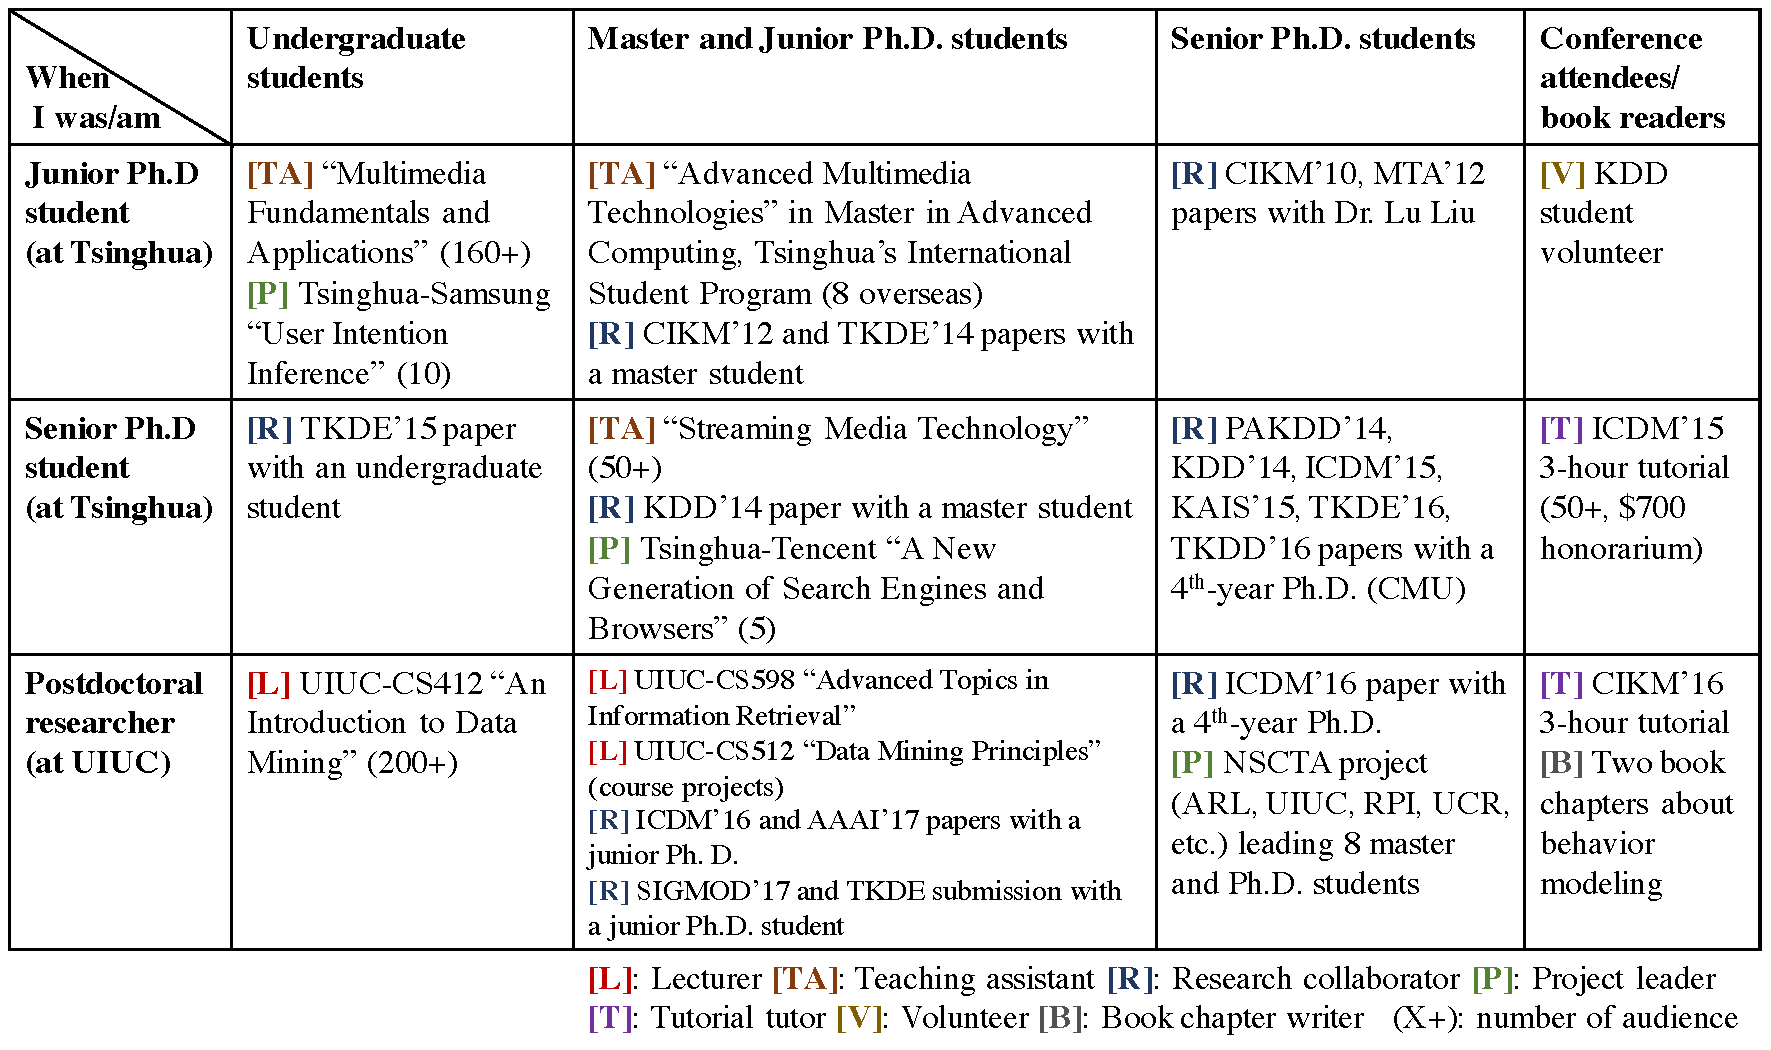
\includegraphics[width=0.7\textwidth]{figure/intro.pdf}
\vskip -0.18in
\caption{My fruitful collaborating, mentoring and teaching experience in the last 7 years.}
\label{fig:intro}
\vskip -0.12in
\end{wrapfigure}

\vskip 0.06in
\noindent {\large \bf 1. Lectures}
\vskip 0.02in

One of the most challenging and fulfilling teaching tasks was delivering lectures. During Fall 2016 I taught fundamental concepts of data mining for the undergraduate-level class \textit{UIUC-CS412 An Introduction to Data Mining} when the instructor Prof. Jiawei Han was out of town. I carefully prepared the lectures to over 200 students on the concept, design and implementation of \textit{Data Warehousing} (DW) as well as the modeling including \textit{Data Cube} and \textit{On-line Analytical Processing} (OLAP)\footnote{\url{https://recordings.engineering.illinois.edu:8443/ess/echo/presentation/7b5971de-3bd5-43f8-9d09-4cdd71649d21}}. First, I watched three related online videos including ones that Prof. Han gave previously. I prepared scripts for each slide and had a few dry run before the lecture. Second, in case that the students were not interested in DW which sounds like an out-of-date concept, I contacted with one of my friends who has taken charge of the DW department of Baidu for six years. I shared his experience in modern industry with the class to emphasize the importance of DW. Third, instead of just pointing to Jim Gray's Data Cube paper, I shared the students with his life experience (e.g., receiving Turing Award, achievements in Microsoft and lost at sea). When the students were more attracted by the theory founder, they were more interested in the theory itself.

In Spring 2016 I gave a lecture on \textit{Enhancing Relationship Prediction with Network Embedding} in the graduate-level class \textit{UIUC-CS512 Data Mining Principles} taught by Prof. Jiawei Han. After it, three groups of students got interested and chose the topic as their course project, one of which was the only group that got A+ from over 20 groups in the project exam.

In Fall 2016 I am going to deliver a guest lecture on \textit{Attribute Discovery from Text} for the graduate-level class \textit{UIUC-CS598 Advanced Topics in Information Retrieval} taught by Prof. Chengxiang Zhai\footnote{UIUC-CS598CXZ schedule. \url{http://times.cs.uiuc.edu/course/598f16/schedule.html}}. The topic is perfectly aligned with a significant part of my research. Making the slides, choosing the right motivating examples, selecting the most relevant state-of-the-art methods, and distilling their essence into a self-contained lecture is extremely valuable. Similarly, I delivered several introductory lectures on \textit{User Behavior Modeling in Social Media} in Tencent Data Seminar, Microsoft Research Asia and University of Massachusetts at Boston.

\vskip 0.06in
\noindent {\large \bf 2. Teaching Assistantships}
\vskip 0.02in

In Tsinghua University, I have served as a Teaching Assistant (TA) for the graduate-level course \textit{Streaming Media Technology} during Fall 2013 taught by Prof. Lifeng Sun for 50+ students, and the undergraduate-level course \textit{Multimedia Fundamentals and Applications} during Spring 2013 taught by Prof. Lianhong Cai for 160+ students. For both courses, I was responsible for (1) designing homework assignments that captured the fundamental concepts and included hands-on experience, (2) holding office hours where I answered questions by the students, and (3) designing research oriented projects for advanced students, and supervising them ensuring the smooth completion of the project. For Tsinghua's International Student \textit{Master in Advanced Computing} Program, I was a TA for the course \textit{Advanced Multimedia Technologies} as well as social activity coordinator for 8 oversea students who come from 6 countries such as Myanmar, Malaysia, Zimbabwe and Malawi. I have enjoyed the focus on ensuring them understand the course material and sharing various cultures. One of the excellent students is now a Ph.D. candidate at University of Melbourne.

\vskip 0.06in
\noindent {\large \bf 3. Tutorials and Book Chapters}
\vskip 0.02in

Conference tutorials are good chances of teaching outside of a university providing comprehensive overviews of a research area. The target audience are researchers and practitioners who may have a working knowledge around the subject matter. I have delivered two tutorials: \textit{Behavioral Modeling in Social Networks: From Micro to Macro}\footnote{ICDM 2015 tutorial. \url{http://www.meng-jiang.com/tutorial-icdm15.html}} \cite{jiang2015behavior} at ICDM 2015 and \textit{Data-Driven Behavioral Analytics: Observations, Representations and Models}\footnote{CIKM 2016 tutorial. \url{http://www.meng-jiang.com/tutorial-cikm16.html}} \cite{jiang2016data} at CIKM 2016. I led the development of both tutorials, including proposing the material, designing the slides and websites, and presenting (all 3 hours at ICDM and 2.5 of 3.5 hours at CIKM). In both cases, the tutorials offered an overview of techniques for modeling behavioral data to support intelligent and trustworthy services such as social recommendation and fraud detection. The ICDM tutorial was well attended, with over 50 participants. I received \$700 honorarium from the conference. Besides the tutorials, I have written two book chapters about behavior modeling for broad readers \cite{jiang2016mining,jiang2016behavior}.

\vskip 0.12in
\noindent {\large \bf II. MENTORING EXPERIENCE}
\vskip 0.02in

I have worked closely with others, and my role in many of my collaborations has been to mentor younger students. I have mentored 1 undergraduate, 2 master students and 2 junior Ph.D. students. These mentorships have led to high quality research. Each of them I supervised has at least one top-tier conference/journal paper accepted (e.g., KDD, TKDE, ICDM, CIKM). The master students have gone on to both Ph.D. programs and industry jobs, and the Ph.D. students have developed into successful independent researchers. Besides the research, I led one large project during each period of my academic life: ``Tsinghua-Samsung'' with 10 undergraduates, ``Tsinghua-Tencent'' with 5 masters and ``UIUC-Army Research Lab'' with 8 Ph.D. students. I was responsible for (1) developing computational models, (2) deploying the models into real systems, and (3) writing final project reports. I encourage student independence and enjoy brainstorming ideas with students, as I have noticed that this is a two-way learning experience. My advising experience at Tsinghua and UIUC has equipped me with the necessary skills to nurture and guide graduate students in my group through their first steps in research, while at the same time having the opportunity to learn from them as well.

\vskip 0.12in
\noindent {\large \bf III. FUTURE TEACHING PLANS}
\vskip 0.02in

I am excited to continue to get exposure and experience with all aspects of communicating, teaching, and mentoring. I would enjoy teaching both fundamental concepts as well as advanced topics and cutting-edge research results. I am qualified and would be happy to teach introductory computer science courses at the undergraduate level. I would be excited to teach courses at any level related to data mining, text mining, data management, databases and machine learning. For more advanced students, I would be delighted to design and teach advanced courses related to my research, such as \textit{User Behavior Modeling} (Prediction, Recommendation and Suspicious Behavior Detection) and \textit{Heterogeneous Information Network Construction and Mining}. Building on my previous teaching and project experience, I strongly believe that at any level, hands-on experience (addressing real-world challenges, manipulating and looking at real data, as well as writing clean and efficient code) is essential both for students interested in working in industry, as well as for students who are more inclined towards a research career, and I will strongly encourage and nurture it. In addition to within-university teaching, I will continue delivering tutorials at conferences, with specific emphasis on cross-disciplinary knowledge, as I have done in the past (adopting behavioral, psychological and social sciences into data-driven models). Finally, drawing from my own experiences, I would be happy to contribute on designing a cross-disciplinary data science curriculum within the school.

\vspace{-0.1in}
%\small{
%\begin{footnotesize}
\bibliographystyle{unsrt}
\bibliography{teaching_statement_jiang}
%\end{footnotesize}
%}

\end{document}


